%%%%%%%%%%%%%%%%%%%%%%%%%%%%%%%%%%%%%%%%%%%%%%%%%%%%%%%%%%%%%%%%%%%%%%%
%%%
%%%         東京理科大学大学院 創域理工学研究科 機械航空宇宙工学専攻
%%%                   【非公式】修士論文要旨 テンプレート
%%%
%%%      <https://github.com/Yuki-MATSUKAWA/TUS-ME_thesis_abstract>
%%%
%%%                                  v1.0.0 Yuki MATSUKAWA 15 Dec. 2021
%%%                                  v2.0.3 Yuki MATSUKAWA 27 Dec. 2023
%%%
%%%%%%%%%%%%%%%%%%%%%%%%%%%%%%%%%%%%%%%%%%%%%%%%%%%%%%%%%%%%%%%%%%%%%%%

\RequirePackage{plautopatch}

% pLaTeX でコンパイルする場合はこれを使う
\documentclass[a4paper,fleqn,dvipdfmx,12pt]{jsarticle}
% upLaTeX でコンパイルする場合はこれを使う
% \documentclass[a4paper,fleqn,dvipdfmx,uplatex,12pt]{jsarticle}

%%% abstract style %%%
% 卒論要旨設定ファイル
\usepackage{master_settings}

% 行番号の表示
% 添削時には行番号を付けるとわかりやすい
% 提出時にはコメントアウトする
% \usepackage[mathlines,pagewise]{lineno}
% \linenumbers\relax

% ページ番号を付けない
\pagestyle{empty}

\begin{document}

% 1 行あたり文字数の指定
\mojiparline{35}
% 1 ページあたり行数の指定
\linesparpage{30}

\begin{center}
% 修士論文題目
ここには修士論文のタイトルを入れます.\\ 一文字でも間違えたら受理されません.
% 修士論文題目
\end{center}

\vskip\baselineskip
\noindent
% 姓と名の間に「全角」スペース忘れずに
\begin{flushright}
    \begin{tabular}{r@{\hspace{3zw}}r@{\hspace{0pt}\vspace{9pt}}}
        機械航空宇宙工学専攻 &
        % 自分の氏名を記入
        % \\ は消さない
        姓姓 名名 \\
        指導教員 &
        % 指導教員の氏名を記入
        姓姓 名名
    \end{tabular}
\end{flushright}

\vskip\baselineskip
%%% ここから書き始める %%%
アブストラクトアブストラクトアブストラクトアブストラクトアブストラクトアブストラクトアブストラクトアブストラクトアブストラクト
アブストラクトアブストラクトアブストラクトアブストラクトアブストラクトアブストラクトアブストラクトアブストラクトアブストラクト
アブストラクトアブストラクトアブストラクトアブストラクトアブストラクトアブストラクトアブストラクトアブストラクトアブストラクト
アブストラクトアブストラクトアブストラクトアブストラクトアブストラクトアブストラクトアブストラクトアブストラクトアブストラクト
アブストラクトアブストラクトアブストラクトアブストラクトアブストラクトアブストラクトアブストラクトアブストラクトアブストラクト
アブストラクトアブストラクトアブストラクトアブストラクトアブストラクトアブストラクトアブストラクトアブストラクトアブストラクト
アブストラクトアブストラクトアブストラクトアブストラクトアブストラクトアブストラクトアブストラクトアブストラクトアブストラクト.

アブストラクトアブストラクトアブストラクトアブストラクトアブストラクトアブストラクトアブストラクトアブストラクトアブストラクト
アブストラクトアブストラクトアブストラクトアブストラクトアブストラクトアブストラクトアブストラクトアブストラクトアブストラクト
アブストラクトアブストラクトアブストラクトアブストラクトアブストラクトアブストラクトアブストラクトアブストラクトアブストラクト
アブストラクトアブストラクトアブストラクトアブストラクトアブストラクトアブストラクトアブストラクトアブストラクトアブストラクト
アブストラクトアブストラクトアブストラクトアブストラクトアブストラクトアブストラクトアブストラクトアブストラクトアブストラクト
アブストラクトアブストラクトアブストラクトアブストラクトアブストラクトアブストラクトアブストラクトアブストラクトアブストラクト
アブストラクトアブストラクトアブストラクトアブストラクトアブストラクトアブストラクトアブストラクトアブストラクトアブストラクト.

図~\ref{fig:abst1}は虎,図~\ref{fig:abst2}も虎.
アブストラクトアブストラクトアブストラクトアブストラクトアブストラクトアブストラクトアブストラクトアブストラクトアブストラクト
アブストラクトアブストラクトアブストラクトアブストラクトアブストラクトアブストラクトアブストラクトアブストラクトアブストラクト
アブストラクトアブストラクトアブストラクトアブストラクトアブストラクトアブストラクトアブストラクトアブストラクトアブストラクト
アブストラクトアブストラクトアブストラクトアブストラクトアブストラクトアブストラクトアブストラクトアブストラクトアブストラクト
アブストラクトアブストラクトアブストラクトアブストラクトアブストラクトアブストラクトアブストラクトアブストラクトアブストラクト
アブストラクトアブストラクトアブストラクトアブストラクトアブストラクトアブストラクトアブストラクトアブストラクトアブストラクト
アブストラクトアブストラクトアブストラクトアブストラクトアブストラクトアブストラクトアブストラクトアブストラクトアブストラクト
アブストラクトアブストラクトアブストラクトアブストラクトアブストラクトアブストラクトアブストラクトアブストラクトアブストラクト
アブストラクトアブストラクトアブストラクトアブストラクトアブストラクトアブストラクト.

\begin{figure}[b]
	\centering
	\begin{minipage}{0.35\columnwidth}
		\centering
		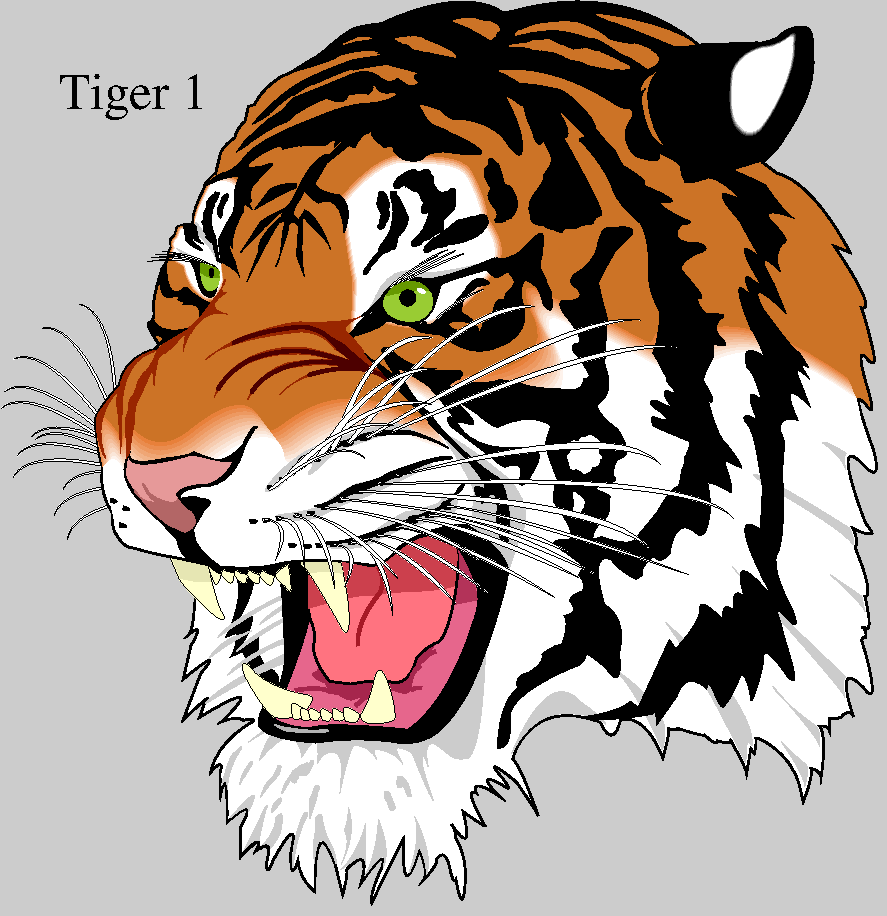
\includegraphics[width=\columnwidth]{tiger1.pdf}
		\caption{Tiger 1.}
		\label{fig:abst1}
	\end{minipage}
	\hspace{15mm}
	\begin{minipage}{0.35\columnwidth}
		\centering
		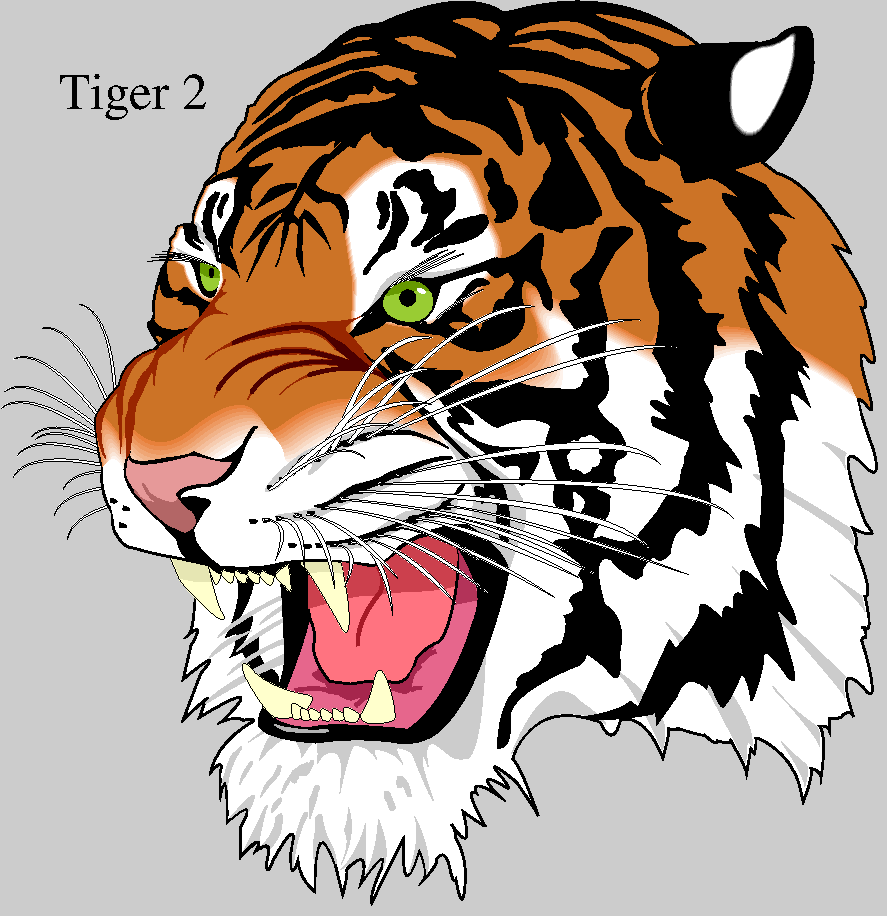
\includegraphics[width=\columnwidth]{tiger2.pdf}
		\caption{Tiger 2.}
		\label{fig:abst2}
	\end{minipage}
\end{figure}

%%% ここまで %%%

\end{document}
